\section{Introduction}
\label{sec:intro}

% Intro structure:
% 1. What is the problem?
% 2. Why is it important?
% 3. Why is the problem hard? What makes it challenging?
% 4. How far has existing work come? Cite a few papers. What is the next frontier?
% 5. Why hasn’t the problem been solved? What is the stumbling block?
% 6. What does our paper contribute?
% 7. What is the key idea? What is the magic trick? What is the new insight or technique that enables us to advance the frontier?
% 8. What do the experiments say?

% 1. What is the problem?
% \cg{(ToDo - add motivation of close range multispectral imaging in forests)}
Forests are essential ecosystems, providing a home to half of all vertebrate species \cite{Pillay2022}, essential ecosystem services, and climate regulation\cite{Brockerhoff2017}. 
Despite their importance, forests are increasingly under threat, from anthropogenic pressures such as logging to the effects of increased climate stress from more frequent extreme weather events and greater susceptibility to invasive pests\cite{FAO2020a}.



% \global\long\def\figHeight{3.3cm}
\begin{figure}[t]
    % \includegraphics[width=\textwidth]{inkscape/eyecatch.png}
    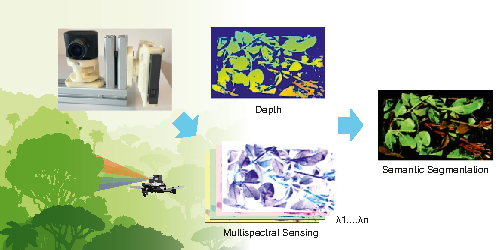
\includegraphics[width=0.5\textwidth]{resources/figures/figure_1_inspiration.pdf}
    \caption{Event Spectroscopy motivation, an all-in-one, ambient-light independent solution for depth sensing, RGB image reconstruction and multispectral sensing. Usable for instance, for an uncrewed aerial vehicle (UAV) navigating in forest environments.  (a) Our setup consisting of an event camera and a projector as an illumination source 
    (b) Depth of scene acquired using structured light (c) RGB image reconstructed from events, (d) Spectral image reconstructed using events (e) Material segmentation of fern leaves using spectral and depth data.} 
    \label{fig:eye} 
\end{figure}


To foster a deeper understanding of the impact of forest ecosystems on biodiversity and the climate it is essential to collect local, high temporal and spatial resolution data, which is currently not feasible in a scalable manner. New technologies and sensing modalities, such as micro aerial vehicles (MAVs) and event cameras present promising solutions to collect this data. MAVs are beginning to demonstrate flights in forests\cite{Loquercio2021, Liu2022}, including for environmental monitoring, such as sensor deployment \cite{Geckeler2022,  Geckeler2023b} or sample collection \cite{Aucone2023a, Charron2020}. These tasks require MAVs to fly in close proximity to tree branches and foliage, where fast-movement and thin branches go beyond the limits of what current conventional sensors can detect for obstacle avoidance and path planning. 
Flying in such close proximity makes interaction with foliage inevitable, and while it has been shown that MAVs can push aside flexible twigs and leaves while avoiding thicker branches\cite{Aucone2024}, proper sensing to differentiate between branches and foliage is needed\cite{Geckeler2024}. This requires not only low latency and high resolution depth sensing of thin and fine structures, but also multispectral sensing to aid in the differentiation between woody branches and foliage.

Once inside the forest canopy, the multispectral data collected by the MAV can also provide invaluable data on tree functioning and physiology. Current methods rely on multispectral data captured from above, either from satellites, aircraft, or MAVs flown above the canopy \cite{Jarocinska2023} and are widespread for tree canopy analysis and species identification \cite{Xu2020a}. The resulting data, however, lacks the spatial resolution to generate specific insights on the individual tree level about tree health and functioning, and is limited to a top-down perspective. To increase the impact of the data it is necessary to collect higher resolution multispectral data, closer to the tree, ideally also from within the canopy. Current passive spectral sensors are strongly dependent on ambient light and the stark lighting intensity changes present below the canopy make application of standard multispectral cameras extremely challenging. An active sensing system that is less reliant on ambient lighting would allow collection of more useful multispectral data from these environments.
% therefore we have active system not dependent on ambient lighting... use for material diff.
%would you need RGB for anything else?

In this work, we propose a single event-based structured light solution which can deliver high-resolution and low latency depth reconstruction with integrated multispectral sensing. 
It is not possible to achieve the aforementioned aims with current sensor solutions, due to inaccurate and slow depth reconstruction and the difficulties of passive spectral data capture under differing illumination conditions. Even setting aside these limitations, a MAV would currently still need to carry multiple conventional sensors; a depth camera for obstacle sensing, an RGB camera for scene video and context, and a multispectral camera to capture multispectral data. Instead, we provide an integrated system utilizing an event camera with structured light to reconstruct high-fidelity depth with low latency. By changing the wavelength of the light used for structured light we can not only reconstruct RGB images, but also perform multispectral sensing by projecting the desired wavelength - with higher resolution and lower latency than available multispectral sensors. First, we demonstrate the quality of our depth reconstruction by showing a XX improvement over other commercial off-the-shelf depth sensors. Next, we demonstrate event-based multispectral sensing using wavelengths between XX in a lab setting and compare our results to a commercial multispectral sensor and a ground truth spectrometer. Furthermore, we demonstrate RGB color image reconstruction using a portable version limited to RGB light projection, as well as material differentiation utilizing both the depth and spectral data on real-world data from a Masoala Rainforest.

% main points%
% - capture high resolution depth + multispectral
% - low latency for dynamic scenes
% - use all info for material differentiation


% Radiance recovery from events has been a challenging task in the event-based vision community.
% Event cameras have the advantage of low-latency, high dynamic range and low bandwidth compared to traditional cameras.
% However, unlike traditional cameras, events do not provide intensity information and therefore, several algorithms have been proposed to convert event steam to intensity data.
% These methods however, only reconstruct intensity but cannot reconstruct spectral information.
% To

%importance of spectral data
% Spectral imaging has applications in remote sensing, environment monitoring, precision agriculture and medical imaging.
% The quality of imaging spectroscopy is evaluated on the following three criteria:
% \begin{itemize}
%     \item Spatial resolution: The smallest possible detail captured by the sensor.
%     \item Spectral resolution: The number of spectral bands a sensor can capture is important as it can result in better quality for material classification.
%     \item Temporal resolution: The duration required for a sensor to capture the same scene with multiple different spectral bands.
% \end{itemize}
% High spectral resolution enables a more detailed analysis of land surfaces, crops and material segmentation.
% Typically this data is captured using a spectrometer that scans a 1D line or 2D plane one spectral band at a time.
% While, achieving a increased spectral resolution, it has a very high latency making it unsuitable for dynamic scenes.
% Inspired by compressive sensing, coded aperture snapshot spectral imager (CASSI) was proposed that captured a 2D multiplexed image of the 3D spectral cube.
% While achieving low-latency, solutions had to be proposed to inverse render the full spectrum data from compressed 2D image.
% To achieve a high spectral and high temporal resolution, we propose an event-based image spectroscopy technique, which takes advantage of the low-latency of the event camera.

% % 6. What does our paper contribute?
% We propose an event-based solution for material segmentation using spectroscopy. 
% Our system consists of a full-spectrum illumination source in combination with rotating bandpass filter in combination with an event camera.
% % The intensity of the scene is recovered by varying the contrast threshold of the event camera.
% With our method, we get depth estimates for free using the principles of structured light for no additional cost to the latency.
% Our experiments show our method achieves $XX$ accuracy in terms of intensity estimation.
% We also show that our depth reconstruction is $XX$ better than any other commerically available depth sensors.
% Additionally, we show the performance of using spectral data and depth for material classification.
% We show that using the depth data improves the performance of our method by $XX$.



\begin{table}[t]
    \centering
    \begin{adjustbox}{max width=\columnwidth}
    \setlength{\tabcolsep}{3pt}
    \begin{tabular}{|c|c|c|c|}
        \toprule
        Sensor & Spatial Resolution & Spectral Resolution & Temporal Resolution \\
        \hline
        Hyperspectral cube \cite{shaw03llj} & & \SI{10}{\nano\meter} &\\
        Multispectral imaging  & & &\\
        CASSI \cite{Wang17PAMI} & & &\\
        Ours & & &\\
    \bottomrule
    \end{tabular}
    \end{adjustbox}
\end{table}